\documentclass[11pt,letterpaper]{article}
\usepackage[margin=0.82in]{geometry}
\usepackage{amsmath,amssymb,bm}
\usepackage{graphicx,booktabs,array}
\usepackage{siunitx}
\usepackage{float}
\usepackage{hyperref}
\usepackage{newtxtext,newtxmath} % Times-like font, appropriate for 11 pt proposal
\usepackage{microtype}
\usepackage{tabularx,booktabs,array}
\usepackage{titlesec}
\usepackage{fancyhdr}
\usepackage{titlesec}
\hypersetup{colorlinks=true,linkcolor=blue,urlcolor=blue}
\sisetup{detect-all}
\title{R16868 Legged Systems\\Problem Set 3: Body Articulation}
\author{Jinwoo Hwang, Ilseung Park}
\date{October 2026}
\begin{document}
\maketitle
\section{Problem 1: Trunk control and apparent virtual pivots}
\subsection*{1. Equation derivation (1.5 points)}
Take $x$ to the right, $z$ upward, and the positive trunk angle $\phi$ to be the orientation whose hip-to-CoM unit vector is $(-\sin\phi,\cos\phi)$. This matches the torque sign in the supplied equations. The CoM, hip, and stance foot obey
\begin{equation}
 \vv r_H = \vv r_C+d(\sin\phi,-\cos\phi)^T,\qquad
 \vv r=\vv r_H-\vv r_{FP}=(x_{rel},z_{rel})^T,\qquad
 l=\|\vv r\|.
 \label{eq:geometry}
\end{equation}
For a compressed spring of rest length $l_0$, define the nonnegative spring force $F_s=k\max(l_0-l,0)$. The spring contributes $\vv F_s=(F_s/l)\vv r$. A torque $\tau$ about the hip creates a reaction force perpendicular to the leg, $\vv F_\tau=(\tau/l^2)(z_{rel},-x_{rel})^T$, because the moment of that force around the stance foot is $x_{rel}F_{\tau,z}-z_{rel}F_{\tau,x}=-\tau$. Thus the total ground reaction on the runner is
\begin{align}
 \vv F_{\mathrm{GRF}} &=\frac{F_s}{l}\begin{bmatrix}x_{rel}\\z_{rel}\end{bmatrix}+
 \frac{\tau}{l^2}\begin{bmatrix}z_{rel}\\-x_{rel}\end{bmatrix},\label{eq:GRF}\\[-0.3em]
 F_x&=\frac{x_{rel}}{l}F_s+\frac{z_{rel}}{l^2}\tau,\qquad
 F_z=\frac{z_{rel}}{l}F_s-\frac{x_{rel}}{l^2}\tau.\label{eq:components}
\end{align}
Translation of the CoM gives $m\ddot x=F_x$ and $m\ddot z=F_z-mg$. The hip lever arm about the CoM is $\vv r_H-\vv r_C=(d\sin\phi,-d\cos\phi)^T$, so its moment is
\begin{equation}
 (\vv r_H-\vv r_C)\times\vv F_{\mathrm{GRF}}
 =d\sin\phi F_z+d\cos\phi F_x.
\end{equation}
Adding the directly applied hip torque gives exactly the specified articulated model:
\begin{equation}
\boxed{\;m\ddot x=F_x,\quad m\ddot z=F_z-mg,\quad
J\ddot\phi=\tau+d(F_x\cos\phi+F_z\sin\phi).\;}
\label{eq:EOM}
\end{equation}
The spring force and torque-induced perpendicular force belong in the stance leg-force computation; Eq.~\eqref{eq:EOM} belongs in the translational/rotational integration block. In flight, $F_s=\tau=F_x=F_z=0$.

\subsection*{2. Load-modulated PD control (2 points)}
With upright reference $\phi_{ref}=0$, the requested controller is
\begin{equation}
\boxed{\quad\tau_{PD}=\frac{F_s}{m}\bigl[K_p(\phi_{ref}-\phi)-K_d\dot\phi\bigr].\quad}
\label{eq:PD}
\end{equation}
The implementation uses $K_p=200$, $K_d=30$ in the force-scaled convention of Eq.~\eqref{eq:PD}; these are illustrative numerical gains rather than values provided by the assignment. The load factor causes the commanded torque to rise during stance compression and decay to zero at liftoff. An unmodulated PD controller could demand hip torque in flight and near zero-load events, causing discontinuous or physically ineffective contact forces. Load modulation also adapts the feedback magnitude to changing normal support, though it does not automatically guarantee stability.

\subsection*{3. Simulink algebraic loop (1 point)}
Insert a \textbf{Memory} block in the feedback path from the computed spring-force signal to the load-modulated PD block. In a fixed-step discrete implementation, a \textbf{Unit Delay} (one integration step) also breaks direct feedthrough. An alternative is to separate the computation of $F_s$ (a function of geometry alone) from the force block receiving $\tau$ so that the solver has no block-level algebraic loop. In the stand-alone numerical implementation, $F_s$ is computed before $\tau$ explicitly and therefore needs no artificial delay.

\subsection*{4. Virtual pivot point torque (5 points)}
The pivot is $h$ above the CoM along the trunk axis, so its position relative to the stance foot is
\begin{align}
\vv r_P-\vv r_{FP}
&=\vv r_H-\vv r_{FP}-(d+h)(\sin\phi,-\cos\phi)^T\\
&=\boxed{\;\vv p=\begin{bmatrix}x_{rel}-(d+h)\sin\phi\\[0.1em] z_{rel}+(d+h)\cos\phi\end{bmatrix}.\;}
\label{eq:p}
\end{align}
Collinearity requires $\vv p\times\vv F_{\mathrm{GRF}}=p_xF_z-p_zF_x=0$. Substitution from Eq.~\eqref{eq:components} yields
\begin{equation}
0=\frac{F_s}{l}(p_x z_{rel}-p_z x_{rel})
 -\frac{\tau}{l^2}(p_x x_{rel}+p_z z_{rel}),
\end{equation}
so that
\begin{equation}
\boxed{\;\tau_{VPP}=
\frac{F_s l (p_xz_{rel}-p_zx_{rel})}{p_xx_{rel}+p_zz_{rel}}
=-\frac{F_s l(d+h)(x_{rel}\cos\phi+z_{rel}\sin\phi)}
 {l^2+(d+h)(z_{rel}\cos\phi-x_{rel}\sin\phi)}.\;}
\label{eq:VPP}
\end{equation}
The implementation takes $h=\SI{0.2}{m}$. The denominator must be nonzero: a singular configuration cannot be regularized without relaxing exact geometric VPP behavior. This formulation commands a torque determined by the instantaneous spring force and leg/trunk geometry, with no freely tuned proportional or derivative gains.

\subsection*{5. Influence of pivot height (1.5 points)}
For a GRF line through $P$, its total moment about the CoM is equivalently the moment of an applied force through $P$:
\begin{equation}
J\ddot\phi=-h\bigl(F_x\cos\phi+F_z\sin\phi\bigr).
\label{eq:pivotmoment}
\end{equation}
For nearly vertical contact force and small $\phi$, this includes a restoring term $-hF_z\phi$. Thus $h>0$ supplies a restoring geometric tendency; $h=0$ eliminates this geometric pitch moment; and $h<0$ reverses its sign and can amplify trunk lean. The actual gait is a hybrid nonlinear system, so bigger positive $h$ need not improve stability: overly strong pitch reactions can drive oscillations or falls.

\begin{figure}[ht]
\centering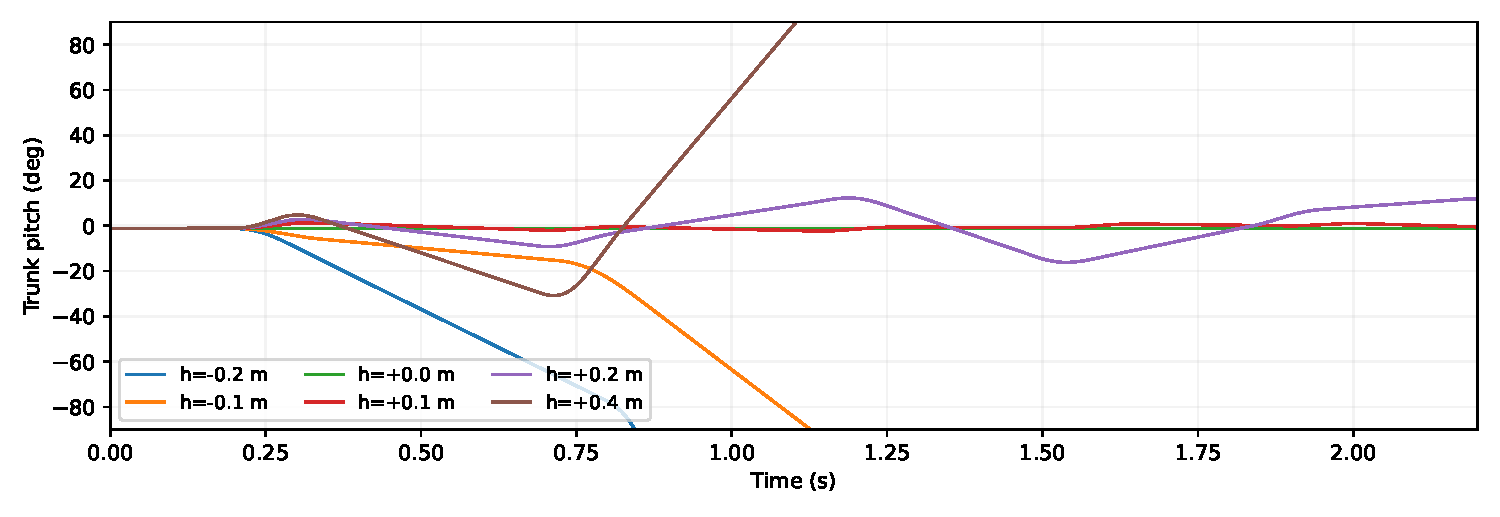
\includegraphics[width=0.97\linewidth]{figures/vpp_height_sensitivity.pdf}
\caption{Pitch responses to prescribed pivot heights, all starting from the same mild initial tilt ($\phi_0=-0.02$ rad). Individual curves end if pitch exceeds $\pi$ radians or the CoM drops below the safety termination height; the truncation is a failure in this simplified simulation, not proof of a general physiological stability boundary.}
\label{fig:h_sweep}
\end{figure}
For the chosen numerical setup, negative $h$ caused the run to terminate early (approximately $\SI{0.96}{s}$ for $h=-0.2$ and $\SI{1.44}{s}$ for $h=-0.1$). The $h=+0.4$ case also terminated early, consistent with excessive response. These are simulation observations for the documented hybrid model, not universal cutoff values.

\subsection*{6. Reducing pitch wobble (1 point)}
Add an angular-velocity damping term, preferably load-modulated so that it vanishes when the spring unloads:
\begin{equation}
\boxed{\quad\tau=\tau_{VPP}-K_{D,VPP}\frac{F_s}{m}\dot\phi.\quad}
\label{eq:damping}
\end{equation}
Here $K_{D,VPP}=10$ is used for illustration. Damping dissipates pitch motion, but its additional force contribution is generally \emph{not} collinear with $\vv p$. Consequently, the GRF lines no longer meet at the originally prescribed pivot exactly; the measured effective pivot can move and become dispersed.

\subsection*{7. Ground-reaction vectors in body coordinates (2 points)}
\paragraph{Coordinate transformation and reproducible simulation.}
With the CoM at the origin, the trunk-fixed basis vectors are $\vv e_{xb}=(\cos\phi,\sin\phi)^T$ and $\vv e_{zb}=(-\sin\phi,\cos\phi)^T$. Define
\begin{equation}
R_{wb}=\begin{bmatrix}\cos\phi&\sin\phi\\-\sin\phi&\cos\phi\end{bmatrix},\quad
\vv r_{FP}^{b}=R_{wb}(\vv r_{FP}^{w}-\vv r_C^{w}),\quad
\vv F^{b}=R_{wb}\vv F^{w}.
\end{equation}
For each stance sample, the plotted line is $\vv r^b(s)=\vv r_{FP}^b+s\hat{\vv F}^b$. To estimate a common intersection, minimize squared perpendicular line distances. With $\vv n_i=(-\hat F_{z,i}^b,\hat F_{x,i}^b)^T$,
\begin{equation}
\vv q_{fit}=\underset{\vv q}{\arg\min}\sum_i
\bigl[\vv n_i^T(\vv q-\vv r_{FP,i}^{b})\bigr]^2,
\qquad e_{RMS}=\sqrt{\tfrac{1}{N}\sum_i\bigl[\vv n_i^T(\vv q_{fit}-\vv r_{FP,i}^{b})\bigr]^2}.
\label{eq:pivotfit}
\end{equation}
The simulations retain the running parameters from the course \texttt{m08\_params.m}: $m=\SI{70}{kg}$, $k=\SI{20000}{N/m}$, $l_0=\SI{1}{m}$, attack angle $68^\circ$, $v_x(0)=\SI{5}{m/s}$, $g=\SI{9.81}{m/s^2}$, and $\Delta t=\SI{1e-4}{s}$. Added articulated parameters are $d=\SI{0.2}{m}$ and $J=\SI{3.5}{kg.m^2}$. The course hip height of $\SI{1.1}{m}$ is retained, meaning $z_C(0)=1.1+d\cos\phi_0$ with $\phi_0=-0.02$ rad. RK4 time integration and a documented single-leg touchdown/liftoff rule are used; this is a stand-alone model initialized from the course parameters, \emph{not} an edited course Simulink file.

\begin{figure}[ht]
\centering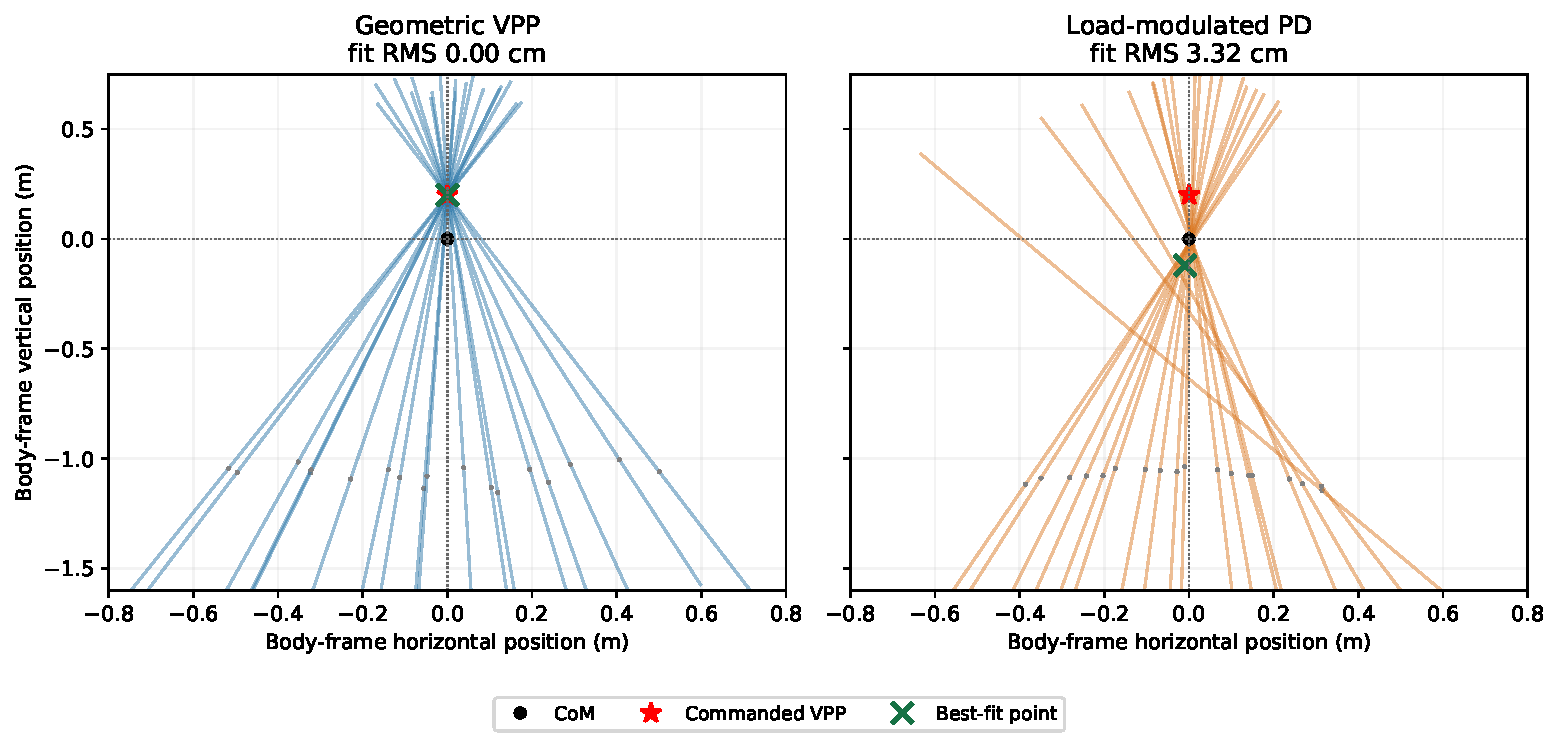
\includegraphics[width=\linewidth]{figures/grf_pivots.pdf}
\caption{Selected stance-phase ground-reaction \emph{lines of action} in the trunk-fixed frame. Black circle: CoM; red star: commanded $h=\SI{0.2}{m}$ pivot; green cross: least-squares effective pivot estimated using all sufficiently loaded stance samples over the full 4-second simulation. The VPP lines intersect exactly at $(0,0.2)$ m; PD exhibits an approximate but non-identical intersection near $(0,-0.119)$ m.}
\label{fig:grf}
\end{figure}
\begin{table}[ht]
\centering
\caption{Numerical pivot estimates. Samples with $F_s>\SI{100}{N}$ were retained.}
\label{tab:pivots}
\begin{tabular}{lrrrr}\toprule
Controller&$N$ samples&$q_x$ (m)&$q_z$ (m)&$e_{RMS}$ (m)\\\midrule
Geometric VPP&15,816&0.0000&0.2000&$6.14\times10^{-16}$\\
Load-modulated PD&15,003&$-0.00946$&$-0.11933$&0.03316\\
VPP + damping&17,285&$-0.00613$&0.11207&0.01980\\\bottomrule
\end{tabular}
\end{table}

\begin{figure}[ht]
\centering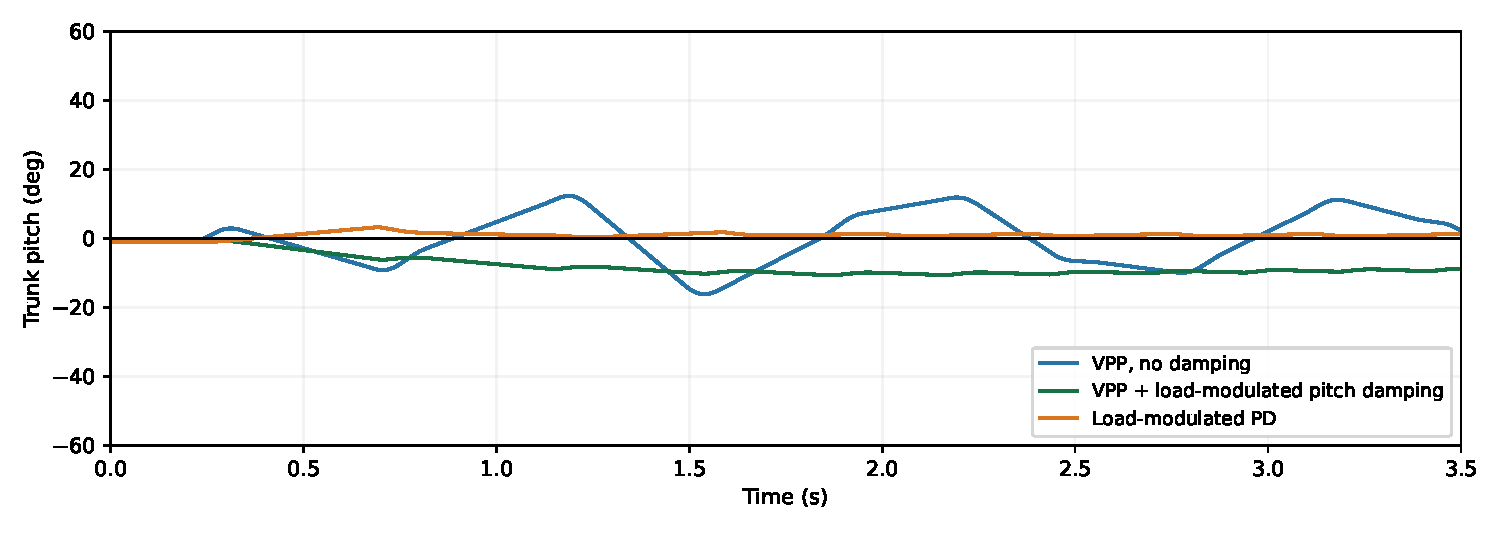
\includegraphics[width=\linewidth]{figures/pitch_comparison.pdf}
\caption{Pitch trajectories for exact VPP, damped VPP ($K_{D,VPP}=10$), and load-modulated PD ($K_p=200,K_d=30$). The controller with damping exhibits less pitch oscillation over this simulated interval, while losing the exact prescribed VPP intersection.}
\label{fig:pitch}
\end{figure}
\paragraph{Interpretation.}
The exact VPP model produces a pivot at $(0,h)$ by construction. The PD model does \emph{not} produce exact line concurrence (about \SI{3.3}{cm} RMS scatter), but its GRFs cluster around a common location even though its controller contains no VPP target. This supports the limited \emph{possibility} that apparent VPP-like patterns can emerge as an observational result of load-aware feedback. It does not demonstrate that animals actually use PD control, nor does it establish that every PD gain choice produces a pivot above the CoM: in this trial, the PD effective pivot lies \emph{below} the CoM. Kinematics, controller gains, and stance selection influence the fitted point.

\subsection*{8. Optional walking extension (2 points): CoP derivation and scope}
When both feet contact the ground, let $\vv F_R=(F_{Rx},F_{Rz})^T$, $\vv F_L=(F_{Lx},F_{Lz})^T$ and their ground-plane positions be $x_{FP,R},x_{FP,L}$. The resultant force and its effective ground-line origin are
\begin{equation}
\vv F_\Sigma=\vv F_R+\vv F_L,\qquad
\boxed{\ x_{CoP}=\frac{x_{FP,R}F_{Rz}+x_{FP,L}F_{Lz}}{F_{Rz}+F_{Lz}},\quad z_{CoP}=0.\ }
\label{eq:cop}
\end{equation}
To compare walking with running, replace each individual force line by $\vv r_{CoP}^b+s\vv F_\Sigma^b$ during double support, use the walking settings ($k=\SI{10000}{N/m}$, attack angle $65^\circ$, $v_x(0)=\SI{1.1}{m/s}$), and fit the effective pivot by Eq.~\eqref{eq:pivotfit}. In single support, the CoP is the stance foot. The resultant line in double support need not pass through either individual stance foot and its direction may depend strongly on the support-force distribution. Thus walking can produce a different apparent VPP height and/or more scatter than running under the same trunk feedback. \textbf{Limitation:} the provided code implements the required \emph{running} model only; no verified two-contact walking simulation was performed, so no numerical walking-versus-running pivot difference is asserted. Equation~\eqref{eq:cop} is the correct analytic method for the optional extension.

\clearpage

\section{Project Proposal}

\subsection{Motivation}
The metatarsophalangeal (MTP) joint allows the forefoot to bend during late stance, shaping heel-to-toe rollover and push-off. Yet many simplified legged robots and walking models use rigid feet. Prior work suggests that toe stiffness can influence walking mechanics and effort~\cite{cho2025,sun2016}, but the relative value of passive articulation and actively controlled toe torque remains dependent on the controller and walking conditions. The key question is: \emph{when does adding a toe joint improve walking, and when is the extra actuation worth its complexity?}

We will test three otherwise identical sagittal-plane bipeds: (i) a rigid foot with the toe hinge locked, (ii) a passive toe with a torsional spring and damper, and (iii) an actuated toe with the same passive elements plus reflex-based torque. We hypothesize that moderate toe compliance can improve rollover and reduce ankle demand, while active toe torque may improve recovery from disturbances at the expense of additional actuator work. These effects will be measured rather than assumed.

\subsection{Planned Effort}
\textbf{Model and controller.} We will develop a two-dimensional biped in MATLAB/Simulink with a torso, bilateral thigh and shank links, and ankle-foot-toe assemblies. Each foot will have heel, forefoot, and toe-tip ground contacts. The articulated toe will use a passive torsional spring and damper; the actuated condition will add bounded reflex torque. Locking the same toe joint will create the rigid-foot baseline, preserving total foot length, segment masses, and contact geometry. The model will use planar rigid-body dynamics and compliant ground contact.
Metabolic cost will be approximated using a joint-work-based estimator
with fixed mechanical efficiency assumptions.

A reflex-inspired controller will use stance loading and trunk-angle feedback for support, ankle torque for propulsion, and phase-dependent hip/knee feedback for swing-leg placement, following the general neuromechanical control approach of Geyer and Herr~\cite{geyer2010}. In the actuated-toe condition, late-stance toe loading and toe angle/velocity will drive a bounded push-off response. Controller structure and feedback inputs will be held constant across conditions. We will first compare identical baseline gains to isolate morphology, then permit limited, equally budgeted gain tuning to assess achievable performance.

\textbf{Evaluation.} After establishing periodic level walking, we will sweep passive toe stiffness and toe-reflex gain.At matched walking speeds, we will compare steady-state rollover
(center-of-pressure progression and toe angle), ankle and toe
mechanical work, positive actuator work per distance, estimated
metabolic cost of transport, and gait failure rate. We will introduce brief torso impulses at consistent gait phases and quantify successful steps and recovery of step timing/forward speed. Toe actuator work will be included when comparing energetic costs. We will report both nominal performance and robustness rather than treating greater toe motion as inherently beneficial.

\subsection*{Weekly timetable}
\vspace{-0.65em}
\renewcommand{\arraystretch}{1.10}
\begin{tabularx}{\linewidth}{@{}>{\raggedright\arraybackslash}p{1.05in}X@{}}
\toprule
\textbf{Dates} & \textbf{Milestone and work}\\
\midrule
Oct 21--27 & Construct and validate the planar walker, toe hinge, and foot-ground contact; test rigid- and passive-foot dynamics.\\
Oct 28--Nov 3 & Implement and tune reflex-inspired hip/knee/ankle control; obtain repeatable rigid-foot level walking.\\
Nov 4--10 & Add passive toe stiffness sweep and actuated toe reflex; verify comparable gait speeds and contact mechanics.\\
Nov 11--17 & Run matched-speed and perturbation experiments; analyze work, rollover, and robustness; prepare report and demonstration.\\
\bottomrule
\end{tabularx}
\vspace{0.3em}

\textbf{Contingency.} If fully autonomous walking is not stable by Week 2, we will simplify the controller and use a stabilizing torso support or prescribed-speed pelvis guidance, retaining dynamic leg/foot contact. In that case, the primary analysis will focus on rollover and joint work; unsupported claims about free-walking stability will be avoided. If active toe control remains unstable, the passive-versus-rigid comparison will remain the core deliverable.

\subsection{Intellectual Merit}
This project will isolate how foot morphology, passive compliance, and fast sensory feedback interact in a hybrid dynamical walking system. Its contribution is a controlled comparison of mechanical and control strategies, not a claim that toe stiffness or toe actuation has never been investigated. By holding geometry and operating conditions comparable, the study can clarify whether improvements arise from compliant rollover, injected toe work, or reflexive adaptation. It will also develop practical understanding of contact mechanics, gait stability, energetic accounting, and neuromechanical feedback control.

\subsection{Broader Impact}
If successful, the results can inform toe-joint design decisions for prosthetic feet, assistive devices, and energy-efficient legged robots: when passive compliance may be sufficient and when active control offers additional value. A reproducible MATLAB/Simulink teaching model will also support hands-on training in multibody dynamics, reflex control, and comparative simulation for future biomechanics and robotics students. As a simplified computational study, it will generate design hypotheses rather than immediate clinical recommendations.

\vspace{-0.35em}
\begin{thebibliography}{9}
\setlength{\itemsep}{0pt}
\setlength{\parskip}{0pt}
\small
\bibitem{cho2025} Cho, K., Lee, K.-W., and Hur, P. (2025). ``Optimizing toe joint stiffness to improve human-like walking.'' \emph{Scientific Reports}, 15, 33268.
\bibitem{sun2016} Sun, S., Huang, Y., and Wang, Q. (2016). ``Adding adaptable toe stiffness affects energetic efficiency and dynamic behaviors of bipedal walking.'' \emph{Journal of Theoretical Biology}, 388, 108--118.
\bibitem{geyer2010} Geyer, H., and Herr, H. (2010). ``A muscle-reflex model that encodes principles of legged mechanics produces human walking dynamics and muscle activities.'' \emph{IEEE Transactions on Neural Systems and Rehabilitation Engineering}, 18(3), 263--273.
\end{thebibliography}

\end{document}